\documentclass{article}
\usepackage{fullpage}
\usepackage[utf8]{inputenc}
\usepackage{pict2e}
\usepackage{amsmath}
\usepackage{enumitem}
\usepackage{eurosym}
\usepackage{mathtools}
\usepackage{amssymb, amsfonts, latexsym, cancel}
\setlength{\parskip}{0.3cm}
\usepackage{graphicx}
\usepackage{fontenc}
\usepackage{slashbox}
\usepackage{setspace}
\usepackage{gensymb}
\usepackage{accents}
\usepackage{adjustbox}
\setstretch{1.35}
\usepackage{bold-extra}
\usepackage[document]{ragged2e}
\usepackage{subcaption}
\usepackage{tcolorbox}
\usepackage{xcolor, colortbl}
\usepackage{wrapfig}
\usepackage{empheq}
\usepackage{array}
\usepackage{parskip}
\usepackage{arydshln}
\graphicspath{ {images/} }
\renewcommand*\contentsname{\color{black}Índice} 
\usepackage{array, multirow, multicol}
\definecolor{lightblue}{HTML}{007AFF}
\usepackage{color}
\usepackage{etoolbox}
\usepackage{listings}
\usepackage{mdframed}
\setlength{\parindent}{0pt}
\usepackage{underscore}
\usepackage{hyperref}
\usepackage{tikz}
\usepackage{tikz-cd}
\usetikzlibrary{shapes, positioning, patterns}
\usepackage{tikz-qtree}
\usepackage{biblatex}
\usepackage{pdfpages}
\usepackage{pgfplots}
\usepackage{pgfkeys}
\addbibresource{biblatex-examples.bib}
\usepackage[a4paper, left=1cm, right=1cm, top=1cm,
bottom=1.5cm]{geometry}
\usepackage{titlesec}
\usepackage{titletoc}
\usepackage{tikz-3dplot}
\usepackage{kbordermatrix}
\usetikzlibrary{decorations.pathreplacing}
\newcommand{\Ej}{\textcolor{lightblue}{\underline{Ejemplo}}}
\setlength{\fboxrule}{1.5pt}

% Configura el formato de las secciones utilizando titlesec
\titleformat{\section}
{\color{red}\normalfont\LARGE\bfseries}
{Tema \thesection:}
{10 pt}
{}

% Ajusta el formato de las entradas de la tabla de contenidos
\addtocontents{toc}{\protect\setcounter{tocdepth}{4}}
\addtocontents{toc}{\color{black}}

\titleformat{\subsection}
{\normalfont\Large\bfseries\color{red}}{\thesubsection)}{1em}{\color{lightblue}}

\titleformat{\subsubsection}
{\normalfont\large\bfseries\color{red}}{\thesubsubsection)}{1em}{\color{lightblue}}

\newcommand{\bboxed}[1]{\fcolorbox{lightblue}{lightblue!10}{$#1$}}
\newcommand{\rboxed}[1]{\fcolorbox{red}{red!10}{$#1$}}

\DeclareMathOperator{\N}{\mathbb{N}}
\DeclareMathOperator{\Z}{\mathbb{Z}}
\DeclareMathOperator{\R}{\mathbb{R}}
\DeclareMathOperator{\Q}{\mathbb{Q}}
\DeclareMathOperator{\K}{\mathbb{K}}
\DeclareMathOperator{\im}{\imath}
\DeclareMathOperator{\jm}{\jmath}
\DeclareMathOperator{\col}{\mathrm{Col}}
\DeclareMathOperator{\fil}{\mathrm{Fil}}
\DeclareMathOperator{\rg}{\mathrm{rg}}
\DeclareMathOperator{\nuc}{\mathrm{nuc}}
\DeclareMathOperator{\dimf}{\mathrm{dimFil}}
\DeclareMathOperator{\dimc}{\mathrm{dimCol}}
\DeclareMathOperator{\dimn}{\mathrm{dimnuc}}
\DeclareMathOperator{\dimr}{\mathrm{dimrg}}
\DeclareMathOperator{\dom}{\mathrm{Dom}}
\DeclareMathOperator{\infi}{\int_{-\infty}^{+\infty}}
\newcommand{\dint}[2]{\int_{#1}^{#2}}

\newcommand{\bu}[1]{\textcolor{lightblue}{\underline{#1}}}
\newcommand{\lb}[1]{\textcolor{lightblue}{#1}}
\newcommand{\db}[1]{\textcolor{blue}{#1}}
\newcommand{\rc}[1]{\textcolor{red}{#1}}
\newcommand{\tr}{^\intercal}

\renewcommand{\CancelColor}{\color{lightblue}}

\newcommand{\dx}{\:\mathrm{d}x}
\newcommand{\dt}{\:\mathrm{d}t}
\newcommand{\dy}{\:\mathrm{d}y}
\newcommand{\dz}{\:\mathrm{d}z}
\newcommand{\dth}{\:\mathrm{d}\theta}
\newcommand{\dr}{\:\mathrm{d}\rho}
\newcommand{\du}{\:\mathrm{d}u}
\newcommand{\dv}{\:\mathrm{d}v}
\newcommand{\tozero}[1]{\cancelto{0}{#1}}
\newcommand{\lbb}[2]{\textcolor{lightblue}{\underbracket[1pt]{\textcolor{black}{#1}}_{#2}}}
\newcommand{\dbb}[2]{\textcolor{blue}{\underbracket[1pt]{\textcolor{black}{#1}}_{#2}}}
\newcommand{\rub}[2]{\textcolor{red}{\underbracket[1pt]{\textcolor{black}{#1}}_{#2}}}

\author{Francisco Javier Mercader Martínez}
\date{}
\title{Procesos Estocásticos y Series Temporales}
\usepackage{amsthm}
\theoremstyle{theorem}
\newtheorem{definition}{Definición}[subsection]
\newtheorem{theorem}{Teorema}[subsection]
\usepackage{framed}
\newenvironment{knitrout}{}{}
\newcolumntype{C}[1]{>{\centering\arraybackslash}p{#1}}
% Colores que knitr suele referenciar
\definecolor{fgcolor}{rgb}{0.345,0.345,0.345}
\definecolor{shadecolor}{rgb}{0.97,0.97,0.97}

\begin{document}
\maketitle
\tableofcontents
\newpage
\section{Introducción a los procesos estocásticos}
Los procesos estocásticos modelizan cantidades numéricas que cambian con el tiempo de manera aleatoria. Ejemplos del mundo real de estos procesos incluyen:
\begin{enumerate}
    \item Resultados sucesivos en un juego de azar.
    \item Número de plazas ocupadas en un parking.
    \item Porcentaje de cielo cubierto en el cielo de Madrid.
    \item Evolución del precio de activos financieros: acciones, tipos de cambio de divisas o criptomonedas, materias primas, etc.
    \item Indicadores económicos como la inflación, el precio de la luz, y el IBEX 35.
\end{enumerate}
Los procesos estocásticos proporcionan marcos matemáticos para modelar y comprender estos fenómenos, lo que permite hacer predicciones y tomar decisiones informadas.

\begin{figure}[h]
\begin{knitrout}
\definecolor{shadecolor}{rgb}{0.969, 0.969, 0.969}\color{fgcolor}

{\centering 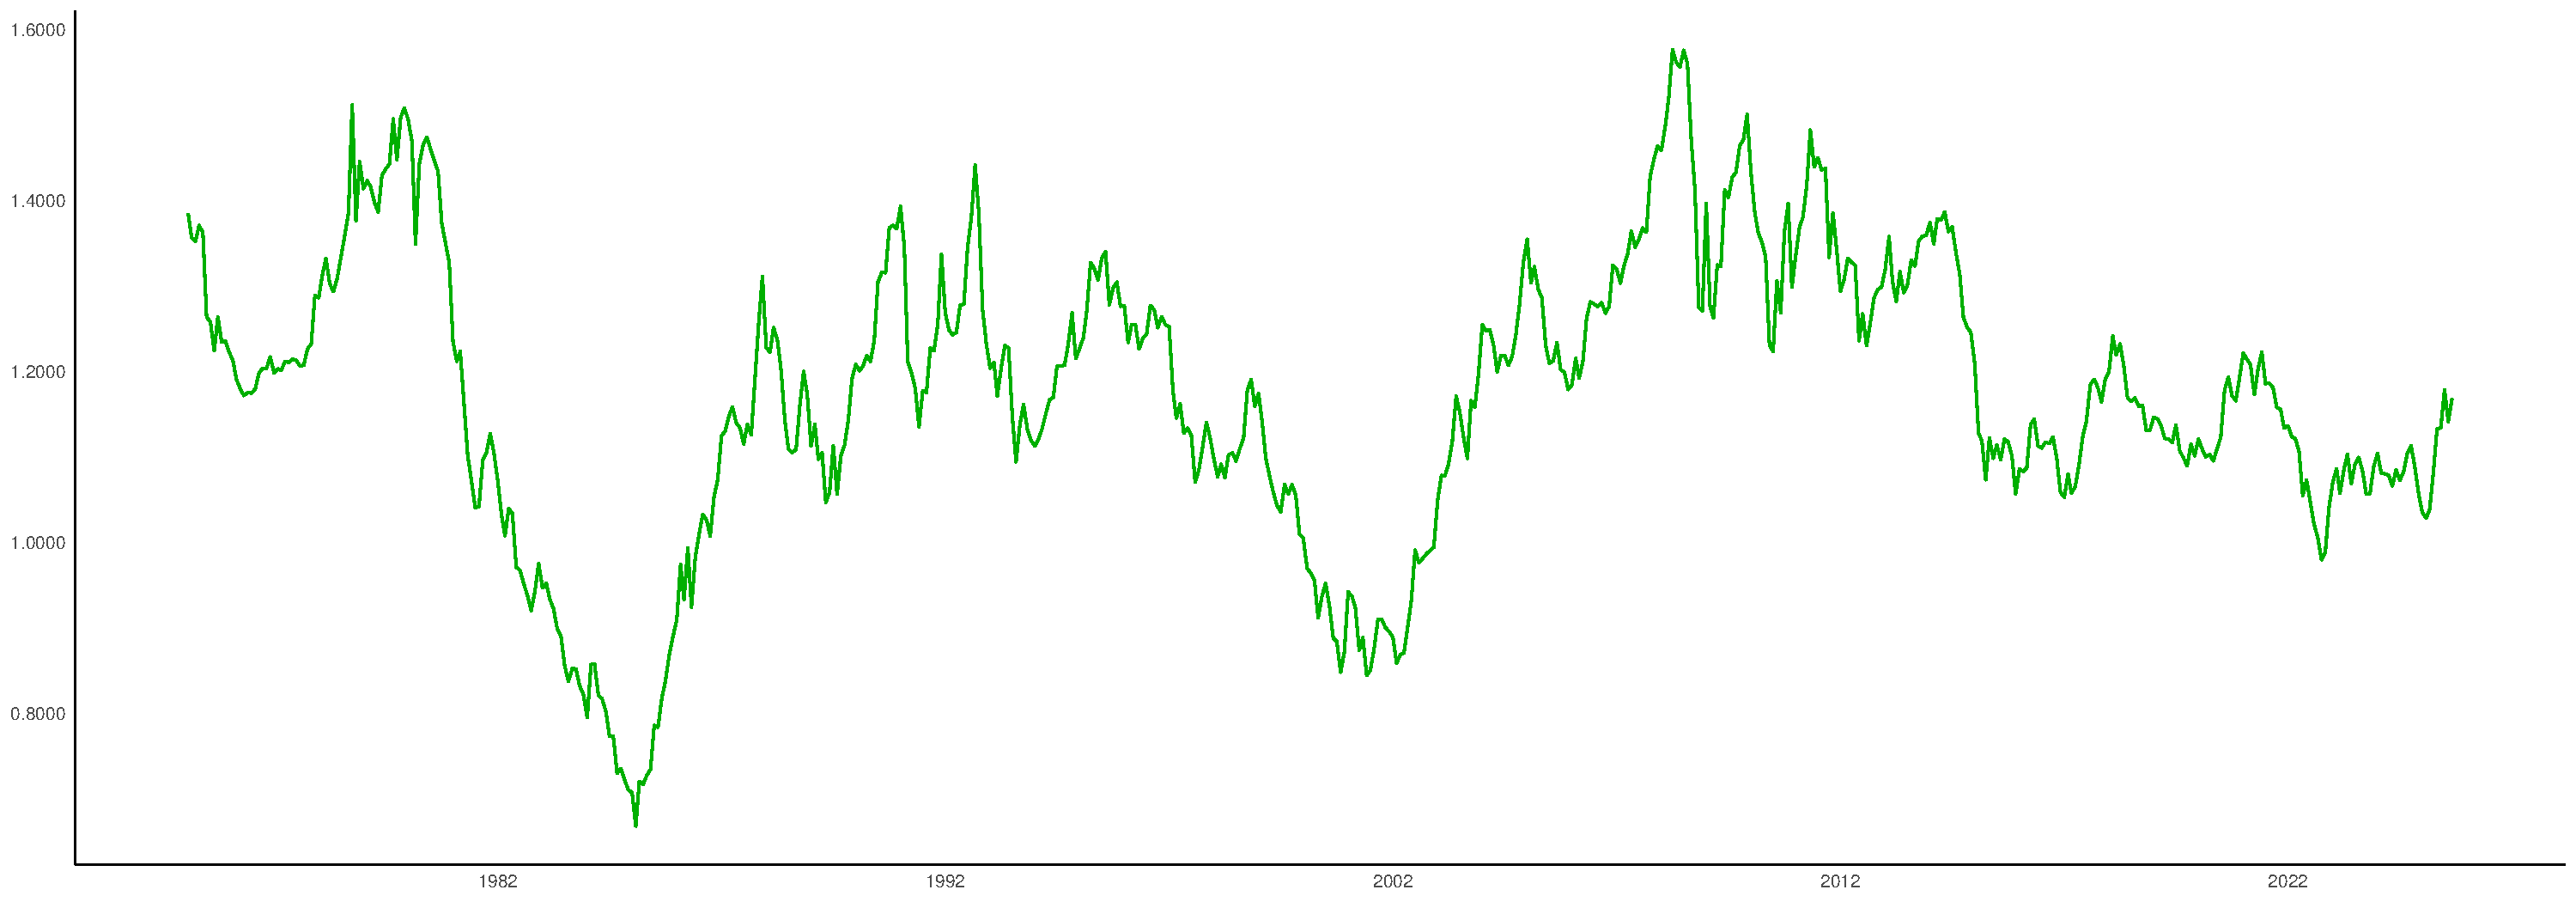
\includegraphics[width=0.7\textwidth]{figure/unnamed-chunk-1-1} 

}


\end{knitrout}
\caption{Evolución del tipo de cambio Euro/dolar (Fuente: Google Finance)}
\end{figure}
\subsection{Concepto de proceso estocástico, trayectorias y ejemplos}
A lo largo de este tema, vamos a fijar un espacio de probabilidad $(\Omega, \mathcal{F}, \mathbb{P})$ y un subconjunto $\mathbb{T}\subset[0,\infty)$.
\begin{definition}
    Un \textbf{proceso estocástico} $(X_t)_{t\in \mathbb{T}}$ es una colección de variables aleatorias reales $X_t$ definidas en el espacio de probabilidad  $(\Omega, \mathcal{F}, \mathbb{P})$.
\end{definition}
Interpretamos $t$ como el tiempo (medido en cierta unidad).
 \begin{itemize}[label=\textbullet]
    \item Si $\mathbb{T}$ es contable (por ejemplo, $\mathbb{T}=\{0<1<2<\dots\} $), diremos que el proceso estocástico $(X_t)_{t\in \mathbb{T}}$ es de tiempo discreto.
    \item Si $\mathbb{T}$ es un intervalo (por ejemplo, $\mathbb{T}=[0,T]$ o $\mathbb{T}=[0,\infty)$), diremos que el proceso estocástico es de tiempo continuo.
\end{itemize}
Para cada $t\in \mathbb{T}$ tenemos una variable aleatoria $X_t$. La variable aleatoria  $X_t$ tomará un valor numérico  $X_t(\omega)$ para cada $\omega\in \Omega$. A los posibles valores que toma un proceso estocástico se les llama \textbf{estados}. 
\begin{itemize}[label=\textbullet]
    \item Si para cada $t\in \mathbb{T}$ la variable aleatoria $X_t$ es de tipo discreto, diremos que el proceso estocástico  $(X_t)_{t\in \mathbb{T}}$ es de estado discreto.
    \item Si para cada $t\in \mathbb{T}$ la variable aleatoria $X_t$ es de tipo continuo, diremos que el proceso estocástico  $(X_t)_{t\in \mathbb{T}}$ es de estado continuo.
\end{itemize}
\newpage
\begin{figure}[h]
    \centering
    \begin{tabular}{|m{2.5cm}|m{4cm}|m{4cm}|}
        \hline
         & $t$ \textbf{Discreto} & $t$  \textbf{Continuo} \\ \hline
    $X$ \textbf{Discreta} & Proceso de estado discreto y tiempo discreto (Unidades prod. mensualmente de un producto) & Proceso de estado discreto y tiempo continuo (Unidades producidas hasta $t$) \\ \hline
$X$ \textbf{Continua} & Proceso de estado continuo y tiempo discreto (Toneladas de producción diaria de un producto) & Proceso de estado continuo y tiempo continuo (Velocidad de un vehículo en el instante $t$) \\ \hline
    \end{tabular}
    \caption{Tipos de procesos estocásticos}
\end{figure}

En lo que sigue, siempre supondremos que $0\in \mathbb{T}$. Esta condición no es realmente restrictiva, ya que podemos desplazar el tiempo por una constante para garantizar que dicha condición se cumple.

\begin{definition}
    Dado un proceso estocástico $(X_t)_{t\in \mathbb{T}}$, para cada realización $\omega\in \Omega$, la colección de números reales $(X_t(\omega))_{t\in \mathbb{T}}$ se llama \textbf{trayectoria} del proceso. 
\end{definition}
\begin{itemize}[label=\textbullet]
    \item Para un proceso estocástico $(X_t)_{t=0,1,2,\dots}$ de tiempo discreto, cada trayectoria define una sucesión de números reales $(x_t)_{t=0,1,2,\dots}$.
    \item Para un proceso estocástico $(X_t)_{t\in [0,\infty)}$ de tiempo continuo, cada trayectoria define una función real $t\mapsto x(t):[0,\infty)\to \R$.
\end{itemize}
Cada trayectoria corresponde a una observación particular de la evolución del valor de un proceso estocástico en el tiempo.

\textbf{Ejemplo.} Supón que inviertes 100 euros en una cuenta bancaria con tipo de interés anual $R$, compuesto anualmente. Es decir, si  $X_t$ es la cantidad de dinero en el año  $t$, entonces  \[
X_t=100\cdot (1+R)^t \text{ para }t=0,1,2,\dots
\]  
Supongamos también que el valor de $R>0$ es fijado cuando metes el dinero en la cuenta y sigue una distribución  $\mathrm{Exp(1)}$.

Para cada observación particular $R=r$ de la variable  $R$ tendremos una trayectoria del proceso estocástico  $(X_t)_{t=0,1,2,\dots}$. Podemos simular y dibujar cinco trayectorias de este proceso estocástico mediante el siguiente código en \textbf{\texttt{R}}: 

\begin{knitrout}
\definecolor{shadecolor}{rgb}{0.969, 0.969, 0.969}\color{fgcolor}

{\centering 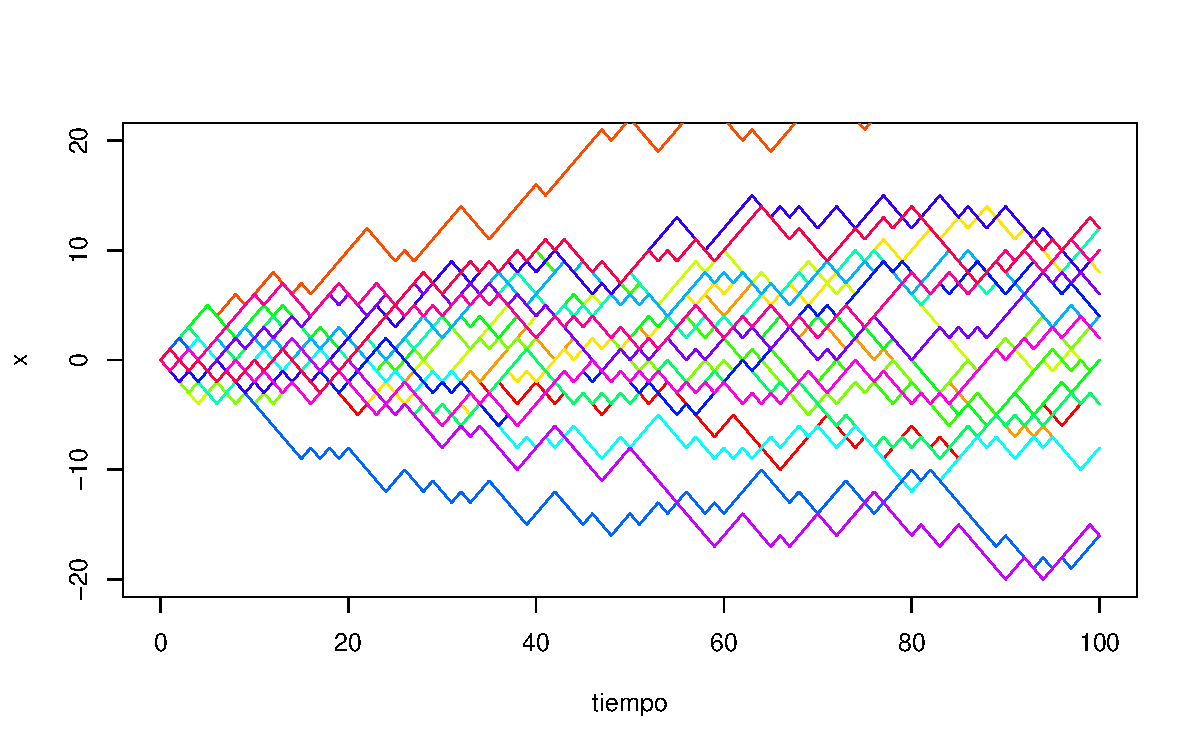
\includegraphics[width=0.7\textwidth]{figure/unnamed-chunk-2-1} 

}


\end{knitrout}

\subsection{Funciones asociadas a un proceso estocástico}

Dado un proceso estocástico $(X_t)_{t\in \mathbb{T}}$, cada variable aleatoria $X_t$ tendrá su propia distribución de probabilidad la cual puede ser discreta o continua. Observar un proceso estocástico en un solo tiempo de forma aislada no es útil para describir su comportamiento como función del tiempo, ya que los valores observados en un tiempo pueden condicionar su comportamiento en tiempos distintos. Por ejemplo, en el caso del camino aleatorio simétrico en el que apostamos un euro a cara, si hemos acumulado muchas ganancias en el pasado, cual disminuirá a lo sumo en un euro en cada lanzamiento.

Por ese motivo, es necesario estudiar la distribución de probabilidad conjunta a lo largo de varios tiempos.
 \begin{definition}
     Supongamos que $(X_t)_{t\in \mathbb{T}}$ es un proceso estocástico. Dada una sucesión finita de tiempos $\{t_1<t_2<\dots<t_n\}\subset \mathbb{T} $, la función $F_{t_1,t_2,\dots,t_n}:\R^n\to [0,1]$ definida por \[
     F_{t_1,t_2,\dots,t_n}(x_1,x_2,\dots,x_n)=\mathbb{P}(X_{t_1}\le x_1,X_{t_2}\le x_2,\dots,X_{t_n}\le x_n),
     \] se llama \textbf{función de distribución (marginal) finito dimensional} del proceso $(X_t)_{t\in \mathbb{T}}$.
\end{definition}
La función de distribución finito dimensional describe el comportamiento probabilístico del proceso estocástico observado en los distintos tiempo $t_1,t_2,\dots,t_n$. La distribución de probabilidad de un proceso está caracterizada por el conjunto de todas las distribuciones finito dimensionales. En particular, dos procesos estocásticos con las mismas funciones de distribución finito dimensionales tendrán un comportamiento probabilístico similar.

En el caso de que $(X_t)_{t\in \mathbb{T}}$ sea de estado discreto, entonces dicho comportamiento probabilístico puede ser descrito por medio la \textbf{función puntual de probabilidad finito dimensional} \[
P_{t_1,t_2,\dots,t_n}(x_1,x_2,\dots,x_n)=\mathbb{P}(X_{t_1}=x_1,X_{t_2}=x_2,\dots,X_{t_n}=x_n).
\] 
En el caso de que $(X_t)_{t\in \mathbb{T}}$ sea de estado continuo, consideramos la \textbf{función de densidad finito dimensional}\newline $f_{t_1,t_2,\dots,t_n}(x_1,x_2,\dots,x_n)$, la cual verifica \[
\mathbb{P}(a_1<X_{t_1}<b_1,\dots,a_n<X_{t_n}<b_n)=\int_{a_n}^{b_n} \cdots \int_{a_1}^{b_1} f_{t_1,t_2,\dots,t_n}(x_1,x_2,\dots,x_n)\dx_1\dots \dx_n  
\] para todo $-\infty\le a_i<b_i\le \infty$.
\begin{definition}
    Dado un proceso estocástico $(X_t)_{t\in \mathbb{T}}$ la \textbf{función medio o función de medias} $\mu_X:\mathbb{T}\to \R$ se define como \[
    \mu_X(t)=\mathbb{E}(X_t).
    \]  
\end{definition}
\begin{itemize}[label=\textbullet]
    \item Para un proceso estocástico $(X_t)_{t=0,1,2,\dots}$ de tiempo discreto, la función media define una sucesión de números reales $(\mu_X(t))_{t=0,1,2,\dots}$ de tiempo discreto, la función media define una sucesión de números reales $(\mu_X(t))_{t=0,1,2,\dots}$.
    \item Para un proceso estocástico $(X_t)_{t\in [0,\infty)}$ de tiempo continuo, la función media define una función real $t \longmapsto \mu_X(t):[0,\infty)\to \R$.
\end{itemize}
La función de medias da una idea de cómo el proceso estocástico se comporta en promedio a lo largo del tiempo.

\textbf{Ejemplo.} Volvamos al ejemplo donde una moneda es lanzada reiteras veces y $(X_t)_{t=0,1,2,\dots}$ son las ganancias acumuladas al apostar un euro a cara en cada lanzamiento (paseo aleatorio simétrico). En este caso, $\mu_X(0)=\mathbb{E}(X_0)=\mathbb{E}(0)=0$ y, si $t>0$,  \[
\mathbb{E}(X_t)=\mathbb{E}(Y_1+Y_2+\dots+Y_t)=\mathbb{E}(Y_1)+\mathbb{E}(Y_2)+\dots+\mathbb{E}(Y_t)=0,
\] donde hemos aplicado que $\mathbb{E}[Y_s]=0$ para todo $s$. En definitiva, la ganancia acumulada promedio es 0 para cualquier número de lanzamientos efectuado.
\begin{definition}
    Dado un proceso estocástico $(X_t)_{t\in \mathbb{T}}$ la \textbf{función de covarianza} $C_X:\mathbb{T}\times \mathbb{T}\to \R$ se define como \[
    C_X(s,t)=\mathrm{Cov}(X_sX_t)=\mathbb{E}\left( (X_s-\mu_X(s))(X_t-\mu_X(t)) \right) =\mathbb{E}(X_sX_t)-\mu_X(s)\mu_X(t).
    \]  
    La \textbf{función de varianza} $\sigma_X^2:\mathbb{T}\to \R$ se define como \[
    \sigma_X^2(t)=\mathrm{Var}(X_t)=C_X(t,t),
    \]  
    y la \textbf{función de correlación} $\rho_X:\mathbb{T}\times \mathbb{T}\to \R$ se define como \[
    \rho_X(s,t)=\dfrac{C_X(s,t)}{\sigma_X(s)\sigma_X(t)}.
    \]  
\end{definition}
\textbf{Ejemplo.} Consideremos el proceso estocástico $(X_t)_{t\in [0,\infty)}$ definido como \[
    X_t=A+Bt\quad\forall t\in [0,\infty),
\] donde $A$ y  $B$ son variables aleatorias  $N(1,1)$ independientes.

Tenemos por un lado que la función de medias viene dada por:  \[
    \mu_X(t)=\mathbb{E}(X_t)=\mathbb{E}(A+Bt)=1+t\quad\forall t\in [0,\infty).
\] 
Y por otro lado la función de varianzas es: \[
C_X(s,t)=\mathbb{E}(X_sX_t)-\mu_X(s)\mu_X(t)
\] 
Observar que la esperanza del producto vale:
\[
\begin{aligned}
    \mathbb{E}(X_sX_t)&= \mathbb{E}\left( (A+Bt)(A+Bs) \right)  \\
                      &= \mathbb{E}(A^2+ABs+ABt+B^2st) \\
                      &= \mathbb{E}(A^2)+\mathbb{E}(A)\mathbb{E}(B)(s+t)+\mathbb{E}(B^2)st \\
                      &= 2+s+t+2st \\
\end{aligned}
\] 
Y el producto de esperanza vale: \[
\mu_X(s)\mu_X(t)=(1+s)(1+t)=1+s+t+st.
\] 
Por tanto, para este proceso estocástico la función de covarianzas es: \[
C_X(s,t)=(2+s+t+2st)-(1+s+t+st)=1+st,
\] la función de varianzas: \[
\sigma_X^2(t)=\mathrm{Var}(X_t)=C_X(t,t)=1+t^2,
\] y la función de correlaciones: \[
\rho_X(s,t)=\dfrac{1+st}{\sqrt{(1+t^2)(1+s^2)} }
\] 
\textbf{Ejemplo.} Volvamos al ejemplo del paseo aleatorio simétrico $(X_t)_{t=0,1,2,\dots}$. Fijados dos números naturales $n,m$ con  $n\le m$, tenemos \[
\begin{aligned}
    C_X(n,m)&=\mathbb{E}\left(X_nX_m\right)\\
            &= \mathbb{E}\left( X_n(X_m-X_n+X_n) \right)  \\
            &= \mathbb{E}\left( X_n(X_m-X_n) \right) +\mathbb{E}\left( X_n^2 \right)  \\
            &= \mathbb{E}(X_n)\mathbb{E}(X_m-X_n)+ \mathbb{E}(X_n^2) \\
            &= n =\min(n,m),\\
\end{aligned}
\] donde hemos usado que $X_n$ y  $X_m-X_n$ son variables aleatorios independientes. Además, obsérvese que, como  $X_n=Y_1+Y_2+\cdots+Y_n$ y las variables $Y_1,Y_2,\dots,Y_n$ son independientes, se tiene que: \[
\mathrm{Var}(X_n)=\mathrm{Var}(Y_1^2)+\mathrm{Var}(Y_2^2)+\cdots+\mathrm{Var}(Y_n^2)=1+1+\cdots+1=n,
\] y por tanto: \[
\mathbb{E}(X_n^2)=\mathrm{Var}(X_n)+(\mathbb{E}(X_n))^2=n+0=n.
\] 
\subsection{Procesos estacionarios y débilmente estacionarios}
Los procesos estocásticos se pueden dividir entre estacionarios (en sentido estricto), débilmente estacionarios y no estacionarios. Intuitivamente hablando, un proceso estocástico es estacionario (en sentido estricto) si su comportamiento probabilístico o distribución no cambia con el tiempo.
\begin{definition}
    Un proceso estocástico $(X_t)_{t\in \mathbb{T}}$ se dice que es \textbf{estacionario} si para toda sucesión finita de tiempos $t_1,t_2,\dots,t_n$ y todo $s>0$ se verifica que los vectores aleatorios  \[
        (X_{t_1},X_{t_2},\dots,X_{t_n})\quad\text{y}\quad(X_{t_1+s},X_{t_2+s},\dots,X_{t_n+s})
    \]  tienen la misma función de distribución, es decir, \[
    F_{t_1,t_2,\dots,t_n}(x_1,x_2,\dots,x_n)=F_{t_1+s,t_2+s,\dots,t_n+s}(x_1,x_2,\dots,x_n)
    \] para cualesquiera números reales $x_1,x_2,\dots,x_n$.
\end{definition}
En particular, si un proceso es estacionario, entonces todas las variables aleatorias $X_t$ del proceso tienen la misma distribución, es decir, están idénticamente distribuidas. Esto no implica que los vectores aleatorios que pueden formar con las variables del proceso en diferentes instantes tengan todos la misma distribución.

En la práctica es muy útil saber si un proceso estocástico es estacionario cuando es necesario predecir el comportamiento futuro de dicho proceso. Si sabemos que el proceso es estacionario, entonces observando su comportamiento en el pasado podremos inferir información de su comportamiento en el futuro.

A continuación introducimos una noción de estacionaridad menos exigente, la cual es también muy útil para predecir comportamientos futuros de procesos estocásticos reales.
 \begin{definition}
    Un proceso estocástico $(X_t)_{t\in \mathbb{T}}$ se dice que es \textbf{débilmente estacionario} si:
    \begin{enumerate}[label=\arabic*)]
        \item $\mu_X(t)=\mu_X(0)$ para todo $t\in \mathbb{T}$. Es decir, la función de medias es constante.
        \item $C_X(s,t)=C_X(0,t-s)$ para todo  $s,t\in \mathbb{T}$ con $s\le t$. Es decir, la función de covarianzas depende sólo del salto entre tiempos.
    \end{enumerate}
\end{definition}
Obsérvese que, en particular, si el proceso es débilmente estacionario tendrá función de varianzas constante.

Dado que la media $\mu_X(t)$ es determinada por la función de distribución marginal $F_t(x)$, y la covarianza  $C_X(s,t)$ es determinada por la función de distribución marginal  $F_{s,t}(x)$, todo proceso estacionario será también débilmente estacionario. Sin embargo, es posible que un proceso sea débilmente estacionario pero no estacionario.

\textbf{Ejemplo.} Consideremos el proceso estocástico $(X_t)_{t\in [0,\infty)}$ definido por \[
X_t=Y\cos(U+t),
\] donde $Y$ y  $U$ son variables aleatorias independientes con  $Y\sim N(0,1)$ y $U\sim U[0,2\pi]$. Entonces \[
\mu_X(t)=0,
\] y además, para $s\le t$, \[
\begin{aligned}
    C_X(s,t)&= \mathbb{E}(X_sX_t)-\mu_X(s)\mu_X(t) \\
    &= \mathbb{E}\left( (Y\cos(U+s))(Y\cos(U+t)) \right)  \\
    &= \mathbb{E}(Y^2)\mathbb{E}\left( \cos(U+s)\cos(U+t) \right)  \\
    &= \mathbb{E}\left( \cos(U+s)\cos(U+t) \right)  \\
    &= \mathbb{E}\left( \frac{1}{2}\cos(2U+s+t)+\frac{1}{2} \cos(t-s)  \right)  \\
    &= \mathbb{E}\left( \frac{1}{2} \cos(2U+s+t) \right)  +\frac{1}{2} \cos(t-s)\\
    &= \dfrac{1}{2} \int_{0}^{2\pi} \left( \cos(2u+s+t)\dfrac{1}{2\pi} \right) \du +\dfrac{1}{2}\cos(t-s) \\
    &= 0+\dfrac{1}{2}\cos(t-s) \\
    &= \dfrac{1}{2}\cos(t-s) \\
\end{aligned}
\] 
En particular, tenemos que $C_X(s,t)=\dfrac{1}{2}\cos(t-s)=C_X(0,t-s)$, de donde deducimos que el proceso estocástico $(X_t)_{t\in [0,\infty)}$ es débilmente estacionario.
\subsection{Procesos gaussianos}
A continuación introducimos una de las familias de procesos estocásticos más importantes: los procesos gaussianos. Este tipo de procesos tienen importantes aplicaciones en Machine Learning.

Recordemos primero la noción de variable \textbf{Normal multivariante}. Una propiedad importante de las variables normales multivariadas es que su función de densidad (y, por tanto, su distribución) está completamente determinada por el sector de medias y la matriz de covarianzas.
\begin{definition}
    Se dice que el vector aleatorio $\vec{X}=(X_1,X_2,\dots,X_n)$ sigue una distribución Normal multivariante si su función de densidad viene dada por: \[
        f_X(\vec{x})=\dfrac{1}{(2\pi)^{\tfrac{n}{2} }\sqrt{|C_X|} }\exp\left\{ -\dfrac{1}{2}(\vec{x}-\vec{\mu}_X)^\intercal C_X^{-1}(\vec{x}-\vec{\mu}_X) \right\} \text{ para todo }\vec{x}\in \R^n,
    \] donde $\vec{\mu}_X$ es el vector de medias de $\vec{X}$ y  $C_X$ es la matriz de covarianzas de  $\vec{X}$.
\end{definition}
\textbf{Propiedad:} Se puede probar, aunque no es inmediato, que una condición equivalente para el vector aleatorio $(X_1,X_2,\dots,X_n)$ siga una distribución Normal multivariante es que, para cualesquiera números reales $a_1,a_2,\dots,a_n$ la variable aleatoria real \[
a_1X_1+a_2X_2+\cdots+a_nX_n
\] sigue una distribución Normal univariante.

Otra importante propiedad de las variables aleatorias normales multivariadas que conviene recordar es que las transformaciones lineales de estas variables también son normales multivariadas. En otras palabras, si $\vec{X}$ es un vector aleatorio Normal multivariante de tamaño  $n,\,A$ es una matriz constante de tamaño  $m\times n$, y $\vec{b}$ es un vector constante de tamaño  $m$, entonces el vector aleatorio  $\vec{Y}=A\vec{X}+\vec{b}$ también es un vector aleatorio Normal multivariante.
 \begin{definition}
    Un proceso estocástico $(X_t)_{t\in \mathbb{T}}$ se dice que es \textbf{gaussiano} (o \textbf{Normal} )  si para toda sucesión de tiempos $t_1,t_2,\dots,t_n\in \mathbb{T}$ el vector aleatorio \[
        (X_{t_1},X_{t_2},\dots,X_{t_n})
    \] es una variable Normal multivariante.
\end{definition}
Una importante propiedad de los procesos gaussianos es que las nociones de estacionaridad y estacionaridad débil son equivalentes para este tipo de procesos. En la práctica esto significa que para verificar que un proceso gaussiano es estacionario basta analizar su media y covarianza. Concretamente, tenemos lo siguiente.
\begin{theorem}
    Sea $(X_t)_{t\in \mathbb{T}}$ un proceso estocástico gaussiano. Si $(X_{t})_{t\in \mathbb{T}}$ es débilmente estacionario, entonces es también estacionario.
\end{theorem}
\newpage
\begin{center}
    \textbf{\Large Hoja 1: Problemas de Introducción a los Procesos Estocásticos} 
\end{center}
\begin{enumerate}[label=\color{red}\textbf{\arabic*)}]
    \item \lb{¿Qué es un proceso estocástico y cómo se define formalmente?}
    \item \lb{¿Cuáles son los tipos principales de procesos estocásticos en función del tiempo?}
    \item \lb{¿Cómo se clasifica un proceso estocástico según los estados que puede formar?} 
\end{enumerate}
\end{document}
